\documentclass{article}
\usepackage[utf8]{inputenc}

\title{Tema 2,Securitate Informației}
\author{Ionită Mihail-Cătălin,Grupa B2}

\usepackage{natbib}
\usepackage{graphicx}
\usepackage{listings}
\usepackage{tikz}

\begin{document}

\maketitle

\section{Exercițiul 1}

Fie următoarele matrici de control al accesului,unde a,b,c,d sunt considerați subiecți.

\begin{center}
\setlength{\tabcolsep}{12pt}
\begin{tabular}{cc}
        \begin{tabular}{|l|l|l|l|} 
        \hline
          & a & b   & c  \\ 
        \hline
        a &   & q   &    \\ 
        \hline
        b & k &     &    \\ 
        \hline
        c & k & q,k &    \\
        \hline
        \end{tabular}
        
        \begin{tabular}{|l|l|l|l|l|} 
        \hline
          & a & b & c & d  \\ 
        \hline
        a &   & t &   &    \\ 
        \hline
        b &   &   & t &    \\ 
        \hline
        c &   &   & q &    \\ 
        \hline
        d &   &   &   &    \\
        \hline
        \end{tabular}
    \end{tabular}
\end{center}

Pentru matricea a) având definită comanda
\begin{center}
    \begin{lstlisting}
    command tansfer(X,Y,Z)
        if q in (X,Y)
        if K in (X,Y)
        if k in (X,Z)
        then
            enter q in (X,Z)
            delete q from (X,Y)
        end
    \end{lstlisting}
\end{center}
a)

Vom descrie in cele ce urmeaza starea matricii de control dupa execuția comenzilor transferq(c,a,b),transferq(c,b,a) 


Vom executa comanda transferq(c,a,b)

Aplicâm pentru $\sigma$(X)=c,$\sigma$(Y)=a și $\sigma$(Z)=b
    \begin{itemize}
        \item verificâm condiția $\sigma$(if q in (X,Y))=if q in (c,a) - fals
        \item verificâm condițtia $\sigma$(if k in (X,Y))=if k in (c,a) -adevărat
        \item verificâm condiția $\sigma$(if k in (X,Z))=if k in (c,b) - adevărat
    \end{itemize}
    \pagebreak
    Cum una dintre condiții este falsă nu se va intra in blocul de instrucțiuni astfel matricea de control al accesului va arata identic cu cea initială
    \begin{center}
        \begin{tabular}{|l|l|l|l|} 
            \hline
              & a & b   & c  \\ 
            \hline
            a &   & q   &    \\ 
            \hline
            b & k &     &    \\ 
            \hline
            c & k & q,k &    \\
            \hline
            \end{tabular}
        \end{center} 
        
        
Vom executa comanda transferq(c,b,a)

Aplicâm pentru $\sigma$(X)=c,$\sigma$(Y)=b și $\sigma$(Z)=a
\begin{itemize}
        \item verificâm condiția $\sigma$(if q in (X,Y))=if q in (c,b) - adevărat
        \item verificâm condițtia $\sigma$(if k in (X,Y))=if k in (c,b) -adevărat
        \item verificâm condiția $\sigma$(if k in (X,Z))=if k in (c,a) - adevărat
        \item aplicâm operațiile
            \begin{itemize}
                \item enter q in ($\sigma$(X),$\sigma$(Z))=(c,a)
                    \begin{itemize}
                        \item $S_1$=S
                        \item $O_1$=O
                        \item $A_1(c,a)$=A(c,a)$\cup${q},$A_1(x,y)=A(x,y)$ dacă x$\neq$c,y$\neq$a
                    \end{itemize}
                \item delete q from ($\sigma$(X),$\sigma$(Y))=(c,b)
                    \begin{itemize}
                        \item $S_2$=$S_1$
                        \item $O_2$=$O_1$
                        \item $A_2(c,b)$=$A_1(c,b)-\{q\}$,$A_1(x,y)=A(x,y)$ dacă x$\neq$c,y$\neq$b
                    \end{itemize}
            \end{itemize}
    \end{itemize}
    Matricea de control al accesului obținută în urma execuției comenzii transferq(c,b,a) este
    \begin{center}
        \begin{tabular}{|l|l|l|l|} 
        \hline
          & a   & b & c  \\ 
        \hline
        a &     & q &    \\ 
        \hline
        b & k   &   &    \\ 
        \hline
        c & q,k & k &    \\
        \hline
        \end{tabular}
    \end{center}

b) 


Definitie: 

Comanda $\alpha$ scurge dreptul r in starea Q dacă:
\begin{itemize}
    \item$\alpha$ se poate aplica stării Q sub p substituție $\sigma$;
    \item prin aplicarea operațiilor comenzii $\alpha$ o celulă a stării Q ce nu conține r ajunge să conțină r
\end{itemize}
    \pagebreak
    Pentru a obține un leak al dreptului q către un nou nod e creat de către nodul a vom aplica comenzile create,grant și take în următoare ordine:
    \begin{enumerate}
        \item b take q for d from c - $take\_q(b,c)$
        \item a take q for d from b - $take\_q(a,b)$
        \item a create t,g for new subject e - $create(a,e)$
        \item a grant q for b to e - $grant\_q(a,e)$
    \end{enumerate}
    
    Astfel în urma aplicării acestor comenzi în celula asociată subiectului e din matricea de control a accesului va apărea dreptul q ceea ce conform definiției este o scurgere a dreptului q.
    
\section{Exercițiul 2}
    Se dă următorul graf take-grant G:
    
    \includegraphics[scale=0.6]{take_grant.jpg}
    
a)Există un span inițial câtre nodul S7 acesta fiind p'=S1 întrucât există tg-drumul S1,S6,S7


b)Pentru a verifica valoarea de adevăr a predicatului can\_share(r,S4,S7,G) vom testa condițiile teoremei 23 prezentate în cadrul cursului

     \includegraphics[scale=0.6]{theorem23.jpg}
     
     Vom verifica condițiile teoremei:
     \pagebreak
     \begin{enumerate}
        \item Cazul I:
            \begin{itemize}
                \item Există o muchie in graful G de la nodul S7 la nodul S4 etichetată cu r - fals
            \end{itemize}
        \item Cazul II:
            \begin{enumerate}
                \item Există un nod s în G,și o muchie de la s la x cu etichetată cu r - Adevărat,s=S5
                \item Există un nod p' în G care fie este chiar p,fie are un span inițial către p, - Adevărat de la subpunctul anterior știm că există un span inițial de la nodul S7 cu p'=S1
                \item Există un nod s' în G care fie este chiar s,fie are un span final către s - Adevărat vom conside cazul în care s=s'=S5 întrucât în sensul original nu există un span final catre s
                \item Nodul p' aparține de o insulă I1,iar s' aparține de o insula In,iar I1 și In sunt conectate fie direct printr-un bridge,fie printr-o cale formată din mai multe bridge-urice trec prin insule intermediare - Fals,putem identifica următoarele insule:
                
                \includegraphics[scale=0.6]{first_island.jpg}
                
                \includegraphics[scale=0.6]{second_island.jpg}
                
                \includegraphics[scale=0.6]{third_island.jpg}
                
                \includegraphics[scale=0.6]{fourth_island.jpg}
                
                
                Între aceste insule nu există  bridge-uri care conectează nodul p' și nodul s',care să respecte definiția structurii de bridge,anume:
                
                Un bridge este un drum care are drept capete două noduri subiect etichetat cu una din secventele:
                \begin{itemize}
                    \item (t)* direția $\rightarrow$
                    \item (t)* direcția $\leftarrow$
                    \item (t)*g(t)* direcțiile $\rightarrow\rightarrow\leftarrow$
                    \item (t)*g(t)* direcțiile $\rightarrow\leftarrow\leftarrow$
                \end{itemize}
                
            \end{enumerate}
     \end{enumerate}
     
     Având în vedere faptul că modelul nu respectă toate condițiile teoremei 23 simultan,putem concluziona faptul că can\_share(r,S4,S7,G)=false
     
\section{Exercițiul 3}

Se dau următoarea diagrame ce exemplifică 
modelarea a doua fluxuri de informație folosind modelele Bell-LaPadula si Biba.
Combinați cele doua diagrame astfel încât direcția fluxului de informație să fie respectat în ceea ce privește clasele cu cea mai mare confidențialitate și cea mai mare integritate.

\includegraphics[scale=0.6]{bell_lapadula.jpg}

Compunerea celor două modele respectând direcția fluxului de informație este următoarea:
\begin{center}
    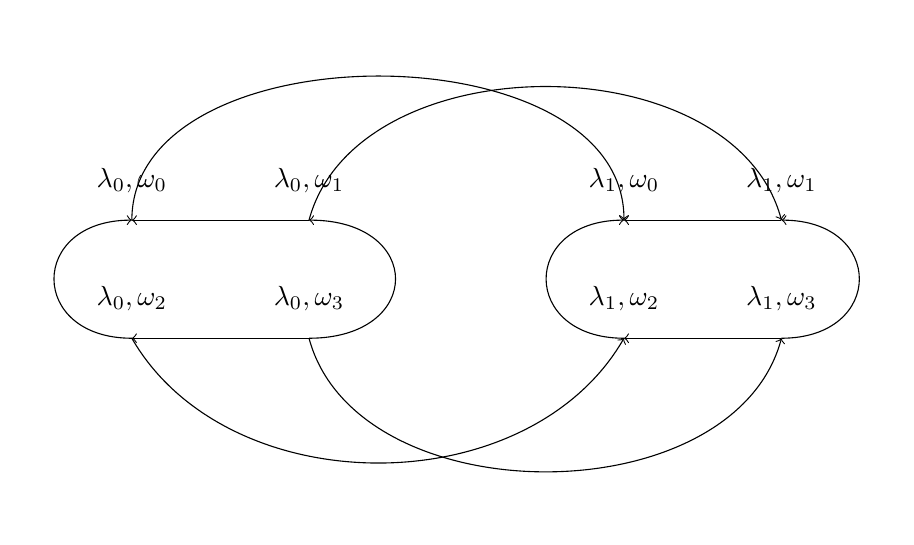
\begin{tikzpicture}

		\node  (0) at (-11, 6) {};
		\node  (1) at (-8.75, 6) {};
		\node  (2) at (-11, 4.5) {};
		\node  (3) at (-8.75, 4.5) {};
		\node  (4) at (-2.75, 4.5) {};
		\node  (5) at (-4.75, 4.5) {};
		\node  (6) at (-2.75, 6) {};
		\node  (7) at (-4.75, 6) {};
		\node  (9) at (-11, 6.5) {$\lambda_0,\omega_0$};
		\node  (10) at (-8.75, 6.5) {$\lambda_0,\omega_1$};
		\node  (11) at (-11, 5) {$\lambda_0,\omega_2$};
		\node  (12) at (-8.75, 5) {$\lambda_0,\omega_3$};
		\node  (13) at (-4.75, 5) {$\lambda_1,\omega_2$};
		\node  (14) at (-2.75, 6.5) {$\lambda_1,\omega_1$};
		\node  (15) at (-4.75, 6.5) {$\lambda_1,\omega_0$};
		\node  (16) at (-2.75, 5) {$\lambda_1,\omega_3$};

		\draw [->](3.center) to (2.center);
		\draw [bend right=90, looseness=2.50,->] (3.center) to (1.center);
		\draw [bend right=270, looseness=2.25,->] (2.center) to (0.center);
		\draw [->](1.center) to (0.center);
		\draw [->](4.center) to (5.center);
		\draw [->](6.center) to (7.center);
		\draw [bend right=270, looseness=2.25,->] (5.center) to (7.center);
		\draw [bend right=90, looseness=2.25,->] (4.center) to (6.center);
		\draw [bend left=90,->] (0.center) to (7.center);
		\draw [bend left=75,->] (1.center) to (6.center);
		\draw [bend right=60,->] (2.center) to (5.center);
		\draw [bend right=75,->] (3.center) to (4.center);
\end{tikzpicture}

\end{center}
\end{document}
